% ═══════════════════════════════════════════════════════════════════════════
% Databricks LaTeX Beamer Presentation - Day 6
% Topic: Medallion Architecture: Complete Guide
% ═══════════════════════════════════════════════════════════════════════════

\documentclass[aspectratio=169]{beamer}

% ─────────────────────────────────────────────────────────────────────────────
% Packages
% ─────────────────────────────────────────────────────────────────────────────
\usepackage{tikz}
\usepackage{graphicx}
\usepackage{hyperref}
\usepackage{xcolor}
\usepackage{fancyhdr}
\usepackage{listings}
\usepackage{tabularx}
\usepackage{booktabs}
\usepackage{fontspec}
\usepackage{amsmath}

\usetikzlibrary{shapes.geometric, arrows.meta, positioning, calc, backgrounds}

% ─────────────────────────────────────────────────────────────────────────────
% Color Definitions - Databricks Palette
% ─────────────────────────────────────────────────────────────────────────────
\definecolor{databricksBlue}{RGB}{41, 49, 66}
\definecolor{databricksRed}{RGB}{220, 53, 69}
\definecolor{databricksYellow}{RGB}{255, 193, 7}
\definecolor{databricksGreen}{RGB}{76, 175, 80}
\definecolor{databricksGray}{RGB}{128, 128, 128}
\definecolor{databricksLightGray}{RGB}{245, 245, 245}
\definecolor{databricksWhite}{RGB}{255, 255, 255}
\definecolor{bronzeColor}{RGB}{205, 127, 50}
\definecolor{silverColor}{RGB}{192, 192, 192}
\definecolor{goldColor}{RGB}{255, 215, 0}

% ─────────────────────────────────────────────────────────────────────────────
% Beamer Theme Configuration
% ─────────────────────────────────────────────────────────────────────────────
\usetheme{default}
\usecolortheme{default}

\setbeamercolor{structure}{fg=databricksBlue}
\setbeamercolor{frametitle}{bg=databricksBlue, fg=white}
\setbeamercolor{title}{fg=white}
\setbeamercolor{subtitle}{fg=databricksLightGray}
\setbeamercolor{author}{fg=databricksLightGray}
\setbeamercolor{institute}{fg=databricksLightGray}
\setbeamercolor{date}{fg=databricksLightGray}
\setbeamercolor{normal text}{fg=databricksBlue}
\setbeamercolor{block title}{bg=databricksBlue, fg=white}
\setbeamercolor{block body}{bg=databricksLightGray, fg=databricksBlue}

\setbeamertemplate{navigation symbols}{}
\setbeamertemplate{itemize item}{\textcolor{databricksBlue}{$\bullet$}}
\setbeamertemplate{itemize subitem}{\textcolor{databricksRed}{$\triangleright$}}
\setbeamertemplate{itemize subsubitem}{\textcolor{databricksGray}{$\circ$}}

% ─────────────────────────────────────────────────────────────────────────────
% Code Listings Configuration
% ─────────────────────────────────────────────────────────────────────────────
\lstset{
    basicstyle=\ttfamily\scriptsize,
    backgroundcolor=\color{databricksLightGray},
    keywordstyle=\color{databricksBlue}\bfseries,
    stringstyle=\color{databricksGreen},
    commentstyle=\color{databricksGray}\itshape,
    breaklines=true,
    frame=single,
    rulecolor=\color{databricksBlue},
    showstringspaces=false,
    tabsize=2
}

% ─────────────────────────────────────────────────────────────────────────────
% Custom Footer with Hyperlinks
% ─────────────────────────────────────────────────────────────────────────────
\setbeamertemplate{footline}{
    \leavevmode%
    \hbox{%
        \begin{beamercolorbox}[wd=.30\paperwidth,ht=2.5ex,dp=1ex,left]{author in head/foot}%
            \usebeamerfont{author in head/foot}\hspace*{2ex}%
            \href{https://easy-ai-labs.lovable.app/}{\textcolor{white}{Easy AI Labs}}
        \end{beamercolorbox}%
        \begin{beamercolorbox}[wd=.40\paperwidth,ht=2.5ex,dp=1ex,center]{title in head/foot}%
            \usebeamerfont{title in head/foot}%
            \href{https://www.linkedin.com/in/yashkavaiya}{\textcolor{white}{Yash Kavaiya}}
        \end{beamercolorbox}%
        \begin{beamercolorbox}[wd=.30\paperwidth,ht=2.5ex,dp=1ex,right]{date in head/foot}%
            \usebeamerfont{date in head/foot}%
            \href{https://www.linkedin.com/company/genai-guru}{\textcolor{white}{Gen AI Guru}}\hspace*{2ex}%
            \textcolor{white}{\insertframenumber{} / \inserttotalframenumber}\hspace*{2ex}
        \end{beamercolorbox}%
    }%
    \vskip0pt%
}

\setbeamercolor{author in head/foot}{bg=databricksBlue}
\setbeamercolor{title in head/foot}{bg=databricksBlue}
\setbeamercolor{date in head/foot}{bg=databricksBlue}

% ─────────────────────────────────────────────────────────────────────────────
% Title Page Template
% ─────────────────────────────────────────────────────────────────────────────
\defbeamertemplate*{title page}{customized}[1][]
{
    \begin{tikzpicture}[remember picture,overlay]
        \fill[databricksBlue] (current page.north west) rectangle (current page.south east);
    \end{tikzpicture}
    \vfill
    \begin{center}
        {\Huge\textcolor{white}{\textbf{\inserttitle}}\par}
        \vspace{0.5cm}
        {\Large\textcolor{databricksYellow}{\insertsubtitle}\par}
        \vspace{1cm}
        {\large\textcolor{databricksLightGray}{\insertauthor}\par}
        \vspace{0.3cm}
        {\normalsize\textcolor{databricksGray}{\insertinstitute}\par}
        \vspace{0.5cm}
        {\small\textcolor{databricksGray}{\insertdate}\par}
    \end{center}
    \vfill
}

% ─────────────────────────────────────────────────────────────────────────────
% Document Information
% ─────────────────────────────────────────────────────────────────────────────
\title{Medallion Architecture}
\subtitle{Complete Guide to Data Quality Layers}
\author{Databricks 14-Days AI Challenge}
\institute{Day 6: Multi-Hop Data Architecture}
\date{\today}

% ═══════════════════════════════════════════════════════════════════════════
% DOCUMENT BEGINS
% ═══════════════════════════════════════════════════════════════════════════
\begin{document}

% Title Slide
\begin{frame}
    \titlepage
\end{frame}

% ─────────────────────────────────────────────────────────────────────────────
% Table of Contents
% ─────────────────────────────────────────────────────────────────────────────
\begin{frame}{Agenda}
    \begin{columns}[T]
        \begin{column}{0.48\textwidth}
            \begin{itemize}
                \item \textcolor{databricksBlue}{\textbf{Introduction}} to Medallion Architecture
                \item \textcolor{databricksBlue}{\textbf{Why}} Medallion Architecture?
                \item \textcolor{bronzeColor}{\textbf{Bronze Layer}}: Raw Data Ingestion
                \item \textcolor{silverColor}{\textbf{Silver Layer}}: Cleaned \& Validated Data
            \end{itemize}
        \end{column}
        \begin{column}{0.48\textwidth}
            \begin{itemize}
                \item \textcolor{goldColor}{\textbf{Gold Layer}}: Business Aggregates
                \item \textcolor{databricksBlue}{\textbf{Data Flow}} \& Transformations
                \item \textcolor{databricksBlue}{\textbf{Incremental Processing}} Patterns
                \item \textcolor{databricksBlue}{\textbf{Best Practices}} for Each Layer
            \end{itemize}
        \end{column}
    \end{columns}
\end{frame}

% ─────────────────────────────────────────────────────────────────────────────
% Introduction to Medallion Architecture
% ─────────────────────────────────────────────────────────────────────────────
\begin{frame}{Introduction to Medallion Architecture}
    \begin{block}{Definition}
        \textbf{Medallion Architecture} (Multi-Hop Architecture) is a data design pattern used to logically organize data in a \textcolor{databricksBlue}{\textbf{lakehouse}}.
    \end{block}
    \vspace{0.3cm}
    \begin{center}
        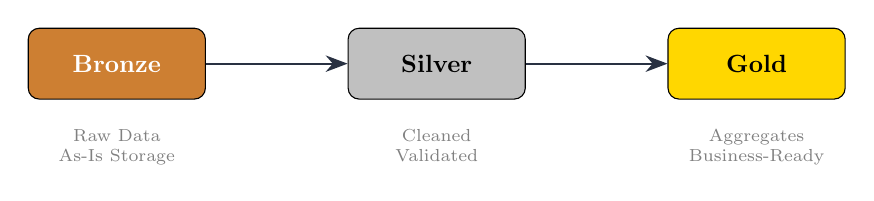
\begin{tikzpicture}[node distance=2cm, scale=0.9, transform shape]
            % Nodes
            \node[draw, fill=bronzeColor, text=white, rounded corners, minimum width=2.5cm, minimum height=1cm] (bronze) {\textbf{Bronze}};
            \node[draw, fill=silverColor, text=black, rounded corners, minimum width=2.5cm, minimum height=1cm, right=of bronze] (silver) {\textbf{Silver}};
            \node[draw, fill=goldColor, text=black, rounded corners, minimum width=2.5cm, minimum height=1cm, right=of silver] (gold) {\textbf{Gold}};
            
            % Labels below
            \node[below=0.3cm of bronze, text=databricksGray, font=\scriptsize, align=center] {Raw Data\\As-Is Storage};
            \node[below=0.3cm of silver, text=databricksGray, font=\scriptsize, align=center] {Cleaned\\Validated};
            \node[below=0.3cm of gold, text=databricksGray, font=\scriptsize, align=center] {Aggregates\\Business-Ready};
            
            % Arrows
            \draw[-{Stealth[scale=1.2]}, thick, databricksBlue] (bronze) -- (silver);
            \draw[-{Stealth[scale=1.2]}, thick, databricksBlue] (silver) -- (gold);
        \end{tikzpicture}
    \end{center}
    \vspace{0.3cm}
    \textcolor{databricksBlue}{\textbf{Principle:}} Data quality and structure improve as data moves from Bronze to Gold.
\end{frame}

% ─────────────────────────────────────────────────────────────────────────────
% Medallion Analogy
% ─────────────────────────────────────────────────────────────────────────────
\begin{frame}{The Refining Analogy}
    \begin{columns}[T]
        \begin{column}{0.30\textwidth}
            \textcolor{databricksBlue}{\textbf{Think of it like refining raw ore:}}
            \begin{itemize}
                \item \textcolor{bronzeColor}{\textbf{Raw ore (Bronze)}}
                \begin{itemize}
                    \item Contains impurities
                    \item Unprocessed material
                \end{itemize}
                \item \textcolor{silverColor}{\textbf{Refined metal (Silver)}}
                \begin{itemize}
                    \item Purified
                    \item Standardized
                \end{itemize}
                \item \textcolor{goldColor}{\textbf{Finished jewelry (Gold)}}
                \begin{itemize}
                    \item Ready for use
                    \item High value
                \end{itemize}
            \end{itemize}
        \end{column}
        \begin{column}{0.70\textwidth}
            \begin{center}
                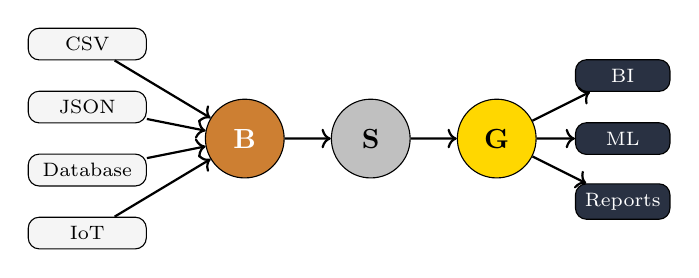
\begin{tikzpicture}[scale=0.8]
                    % Sources
                    \node[draw, fill=databricksLightGray, rounded corners, minimum width=1.5cm, font=\scriptsize] at (0,3) (csv) {CSV};
                    \node[draw, fill=databricksLightGray, rounded corners, minimum width=1.5cm, font=\scriptsize] at (0,2) (json) {JSON};
                    \node[draw, fill=databricksLightGray, rounded corners, minimum width=1.5cm, font=\scriptsize] at (0,1) (db) {Database};
                    \node[draw, fill=databricksLightGray, rounded corners, minimum width=1.5cm, font=\scriptsize] at (0,0) (iot) {IoT};
                    
                    % Layers
                    \node[draw, fill=bronzeColor, text=white, circle, minimum size=1cm] at (2.5,1.5) (b) {\textbf{B}};
                    \node[draw, fill=silverColor, text=black, circle, minimum size=1cm] at (4.5,1.5) (s) {\textbf{S}};
                    \node[draw, fill=goldColor, text=black, circle, minimum size=1cm] at (6.5,1.5) (g) {\textbf{G}};
                    
                    % Consumers
                    \node[draw, fill=databricksBlue, text=white, rounded corners, minimum width=1.2cm, font=\scriptsize] at (8.5,2.5) (bi) {BI};
                    \node[draw, fill=databricksBlue, text=white, rounded corners, minimum width=1.2cm, font=\scriptsize] at (8.5,1.5) (ml) {ML};
                    \node[draw, fill=databricksBlue, text=white, rounded corners, minimum width=1.2cm, font=\scriptsize] at (8.5,0.5) (rpt) {Reports};
                    
                    % Arrows
                    \foreach \src in {csv, json, db, iot} \draw[->, thick] (\src) -- (b);
                    \draw[->, thick] (b) -- (s);
                    \draw[->, thick] (s) -- (g);
                    \foreach \dst in {bi, ml, rpt} \draw[->, thick] (g) -- (\dst);
                \end{tikzpicture}
            \end{center}
        \end{column}
    \end{columns}
\end{frame}

% ─────────────────────────────────────────────────────────────────────────────
% Why Medallion Architecture?
% ─────────────────────────────────────────────────────────────────────────────
\begin{frame}{Why Medallion Architecture?}
    \begin{columns}[T]
        \begin{column}{0.48\textwidth}
            \textcolor{databricksRed}{\textbf{Problems It Solves:}}
            \vspace{0.3cm}
            \begin{itemize}
                \item \textcolor{databricksBlue}{\textbf{Data Quality Issues}}
                \begin{itemize}
                    \item Progressive refinement
                \end{itemize}
                \item \textcolor{databricksBlue}{\textbf{Debugging Difficulties}}
                \begin{itemize}
                    \item Raw data preserved in Bronze
                \end{itemize}
                \item \textcolor{databricksBlue}{\textbf{Schema Changes}}
                \begin{itemize}
                    \item Transformations in Silver
                \end{itemize}
                \item \textcolor{databricksBlue}{\textbf{Reprocessing Needs}}
                \begin{itemize}
                    \item Replay from Bronze
                \end{itemize}
            \end{itemize}
        \end{column}
        \begin{column}{0.48\textwidth}
            \textcolor{databricksGreen}{\textbf{Key Benefits:}}
            \vspace{0.3cm}
            \begin{enumerate}
                \item \textbf{Data Lineage} - Traceable transformations
                \item \textbf{Replayability} - Reprocess without re-ingesting
                \item \textbf{Separation of Concerns} - Clear responsibilities
                \item \textbf{Quality Gates} - Validation at each layer
                \item \textbf{Flexibility} - Multiple Gold tables
                \item \textbf{Performance} - Pre-aggregated queries
            \end{enumerate}
        \end{column}
    \end{columns}
\end{frame}

% ─────────────────────────────────────────────────────────────────────────────
% The Three Layers Overview
% ─────────────────────────────────────────────────────────────────────────────
\begin{frame}{The Three Layers at a Glance}
    \begin{center}
    \scriptsize
    \begin{tabular}{l|c|c|c}
        \toprule
        \textbf{Aspect} & \textcolor{bronzeColor}{\textbf{Bronze}} & \textcolor{silverColor}{\textbf{Silver}} & \textcolor{goldColor}{\textbf{Gold}} \\
        \midrule
        Data Quality & Raw, may have issues & Cleaned, validated & Aggregated, business-ready \\
        Schema & Schema-on-read & Schema enforced & Highly structured \\
        Duplicates & May exist & Removed & N/A (aggregated) \\
        Transformations & None (only metadata) & Filtering, cleaning & Aggregations \\
        Users & Data engineers & Engineers, analysts & Business users, BI \\
        Update Pattern & Append-only & Upsert/Merge & Overwrite or Merge \\
        \bottomrule
    \end{tabular}
    \end{center}
\end{frame}

% ─────────────────────────────────────────────────────────────────────────────
% Bronze Layer Introduction
% ─────────────────────────────────────────────────────────────────────────────
\begin{frame}{Bronze Layer: Raw Data Ingestion}
    \begin{columns}[T]
        \begin{column}{0.48\textwidth}
            \begin{block}{\textcolor{bronzeColor}{What is the Bronze Layer?}}
                The \textbf{landing zone} for all raw data. Captures data exactly as received with minimal transformation.
            \end{block}
            \vspace{0.3cm}
            \textcolor{databricksBlue}{\textbf{Characteristics:}}
            \begin{itemize}
                \item Raw and Unmodified
                \item Append-Only pattern
                \item Full History preserved
                \item Metadata Enriched
                \item Schema-on-Read
            \end{itemize}
        \end{column}
        \begin{column}{0.48\textwidth}
            \textcolor{databricksBlue}{\textbf{Formula:}}
            \begin{center}
                \fcolorbox{databricksBlue}{databricksLightGray}{
                    \parbox{0.85\textwidth}{
                        \centering
                        \texttt{Source Data + Metadata = Bronze}
                    }
                }
            \end{center}
            \vspace{0.3cm}
            \textcolor{databricksBlue}{\textbf{Common Metadata Fields:}}
            \begin{itemize}
                \item \texttt{ingestion\_timestamp}
                \item \texttt{source\_file}
                \item \texttt{source\_system}
                \item \texttt{batch\_id}
            \end{itemize}
        \end{column}
    \end{columns}
\end{frame}

% ─────────────────────────────────────────────────────────────────────────────
% Bronze Layer Code
% ─────────────────────────────────────────────────────────────────────────────
\begin{frame}[fragile]{Bronze Layer: Code Example}
\begin{lstlisting}[language=Python, caption=Bronze Layer Ingestion]
# BRONZE: Raw ingestion
raw = spark.read.csv(
    "/raw/events.csv",
    header=True,
    inferSchema=True
)

# Add metadata and save to Bronze
raw.withColumn("ingestion_ts", F.current_timestamp()) \
   .write.format("delta") \
   .mode("overwrite") \
   .save("/delta/bronze/events")
\end{lstlisting}
    \vspace{0.3cm}
    \begin{center}
        \scriptsize
        \begin{tabular}{l|l}
            \toprule
            \textbf{Code Element} & \textbf{Purpose} \\
            \midrule
            \texttt{header=True} & First row contains column names \\
            \texttt{inferSchema=True} & Auto-detect data types \\
            \texttt{ingestion\_ts} & When data was ingested \\
            \texttt{format("delta")} & ACID transactions enabled \\
            \bottomrule
        \end{tabular}
    \end{center}
\end{frame}

% ─────────────────────────────────────────────────────────────────────────────
% Bronze Layer Best Practices
% ─────────────────────────────────────────────────────────────────────────────
\begin{frame}{Bronze Layer: Best Practices}
    \begin{center}
    \begin{tabular}{l|l|l}
        \toprule
        \textbf{Practice} & \textbf{Description} & \textbf{Reason} \\
        \midrule
        \textcolor{databricksGreen}{Never modify raw data} & Store as received & Audit trails \\
        \textcolor{databricksGreen}{Use append mode} & Add, don't overwrite & Preserve history \\
        \textcolor{databricksGreen}{Add ingestion metadata} & Timestamp, source & Debugging \\
        \textcolor{databricksGreen}{Partition by date} & Ingestion date & Efficient processing \\
        \textcolor{databricksGreen}{Keep original schema} & Don't rename columns & Source comparison \\
        \textcolor{databricksGreen}{Use Delta format} & ACID, time travel & Reliability \\
        \bottomrule
    \end{tabular}
    \end{center}
\end{frame}

% ─────────────────────────────────────────────────────────────────────────────
% Silver Layer Introduction
% ─────────────────────────────────────────────────────────────────────────────
\begin{frame}{Silver Layer: Cleaned and Validated Data}
    \begin{columns}[T]
        \begin{column}{0.48\textwidth}
            \begin{block}{\textcolor{silverColor}{What is the Silver Layer?}}
                Contains \textbf{cleaned, validated, and enriched data}. Quality rules applied, duplicates removed.
            \end{block}
            \vspace{0.3cm}
            \textcolor{databricksBlue}{\textbf{Characteristics:}}
            \begin{itemize}
                \item Cleaned Data
                \item Validated (business rules)
                \item Deduplicated
                \item Enriched (derived columns)
                \item Schema Enforced
                \item Joined (multiple sources)
            \end{itemize}
        \end{column}
        \begin{column}{0.48\textwidth}
            \textcolor{databricksBlue}{\textbf{Common Operations:}}
            \begin{center}
                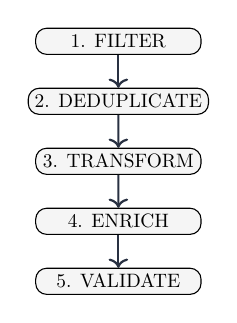
\begin{tikzpicture}[node distance=0.6cm, scale=0.7, transform shape]
                    \node[draw, fill=databricksLightGray, rounded corners, minimum width=3cm] (f) {1. FILTER};
                    \node[draw, fill=databricksLightGray, rounded corners, minimum width=3cm, below=of f] (d) {2. DEDUPLICATE};
                    \node[draw, fill=databricksLightGray, rounded corners, minimum width=3cm, below=of d] (t) {3. TRANSFORM};
                    \node[draw, fill=databricksLightGray, rounded corners, minimum width=3cm, below=of t] (e) {4. ENRICH};
                    \node[draw, fill=databricksLightGray, rounded corners, minimum width=3cm, below=of e] (v) {5. VALIDATE};
                    
                    \draw[->, thick, databricksBlue] (f) -- (d);
                    \draw[->, thick, databricksBlue] (d) -- (t);
                    \draw[->, thick, databricksBlue] (t) -- (e);
                    \draw[->, thick, databricksBlue] (e) -- (v);
                \end{tikzpicture}
            \end{center}
        \end{column}
    \end{columns}
\end{frame}

% ─────────────────────────────────────────────────────────────────────────────
% Silver Layer Code
% ─────────────────────────────────────────────────────────────────────────────
\begin{frame}[fragile]{Silver Layer: Code Example}
\begin{lstlisting}[language=Python, caption=Silver Layer Cleaning]
# SILVER: Cleaned data
bronze = spark.read.format("delta").load("/delta/bronze/events")

silver = bronze \
    .filter(F.col("price") > 0) \
    .filter(F.col("price") < 10000) \
    .dropDuplicates(["user_session", "event_time"]) \
    .withColumn("event_date", F.to_date("event_time")) \
    .withColumn("price_tier",
        F.when(F.col("price") < 10, "budget")
         .when(F.col("price") < 50, "mid")
         .otherwise("premium"))

silver.write.format("delta").mode("overwrite") \
      .save("/delta/silver/events")
\end{lstlisting}
\end{frame}

% ─────────────────────────────────────────────────────────────────────────────
% Silver Layer Code Breakdown
% ─────────────────────────────────────────────────────────────────────────────
\begin{frame}{Silver Layer: Code Breakdown}
    \begin{center}
    \scriptsize
    \begin{tabular}{l|l|l}
        \toprule
        \textbf{Operation} & \textbf{Code} & \textbf{Purpose} \\
        \midrule
        \textcolor{databricksRed}{Validation} & \texttt{filter(price > 0)} & Remove invalid prices \\
        \textcolor{databricksRed}{Validation} & \texttt{filter(price < 10000)} & Remove outliers \\
        \textcolor{databricksBlue}{Deduplication} & \texttt{dropDuplicates([...])} & One record per session \\
        \textcolor{databricksGreen}{Transformation} & \texttt{to\_date("event\_time")} & Extract date \\
        \textcolor{databricksYellow}{Enrichment} & \texttt{F.when(...)} & Categorize prices \\
        \bottomrule
    \end{tabular}
    \end{center}
    \vspace{0.5cm}
    \textcolor{databricksBlue}{\textbf{Price Tier Logic:}}
    \begin{center}
    \begin{tabular}{l|l}
        \toprule
        \textbf{Price Range} & \textbf{Tier} \\
        \midrule
        \$0.01 - \$9.99 & budget \\
        \$10.00 - \$49.99 & mid \\
        \$50.00+ & premium \\
        \bottomrule
    \end{tabular}
    \end{center}
\end{frame}

% ─────────────────────────────────────────────────────────────────────────────
% Silver Layer Best Practices
% ─────────────────────────────────────────────────────────────────────────────
\begin{frame}{Silver Layer: Best Practices}
    \begin{center}
    \begin{tabular}{l|l}
        \toprule
        \textbf{Practice} & \textbf{Description} \\
        \midrule
        \textcolor{databricksGreen}{Document business rules} & Record why each filter exists \\
        \textcolor{databricksGreen}{Handle nulls explicitly} & Filter, fill default, or keep \\
        \textcolor{databricksGreen}{Use meaningful names} & Rename cryptic columns \\
        \textcolor{databricksGreen}{Standardize formats} & Consistent dates, units \\
        \textcolor{databricksGreen}{Add quality flags} & Indicators for cleaned records \\
        \textcolor{databricksGreen}{Partition appropriately} & Usually by business date \\
        \textcolor{databricksGreen}{Enable schema enforcement} & Use Delta schema evolution \\
        \bottomrule
    \end{tabular}
    \end{center}
\end{frame}

% ─────────────────────────────────────────────────────────────────────────────
% Gold Layer Introduction
% ─────────────────────────────────────────────────────────────────────────────
\begin{frame}{Gold Layer: Business Aggregates}
    \begin{columns}[T]
        \begin{column}{0.48\textwidth}
            \begin{block}{\textcolor{goldColor}{What is the Gold Layer?}}
                Contains \textbf{business-level aggregates and metrics} ready for consumption by analysts and BI tools.
            \end{block}
            \vspace{0.3cm}
            \textcolor{databricksBlue}{\textbf{Characteristics:}}
            \begin{itemize}
                \item Pre-aggregated
                \item Business-Focused
                \item Consumption-Ready
                \item Multiple Domain Tables
                \item Denormalized
            \end{itemize}
        \end{column}
        \begin{column}{0.48\textwidth}
            \textcolor{databricksBlue}{\textbf{Example Gold Tables:}}
            \begin{center}
                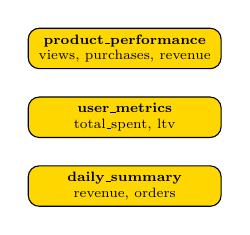
\begin{tikzpicture}[node distance=0.5cm, scale=0.7, transform shape]
                    \node[draw, fill=goldColor, rounded corners, minimum width=3.5cm, align=center, font=\scriptsize] (p) {\textbf{product\_performance}\\views, purchases, revenue};
                    \node[draw, fill=goldColor, rounded corners, minimum width=3.5cm, align=center, font=\scriptsize, below=of p] (u) {\textbf{user\_metrics}\\total\_spent, ltv};
                    \node[draw, fill=goldColor, rounded corners, minimum width=3.5cm, align=center, font=\scriptsize, below=of u] (d) {\textbf{daily\_summary}\\revenue, orders};
                \end{tikzpicture}
            \end{center}
        \end{column}
    \end{columns}
\end{frame}

% ─────────────────────────────────────────────────────────────────────────────
% Gold Layer Code
% ─────────────────────────────────────────────────────────────────────────────
\begin{frame}[fragile]{Gold Layer: Code Example}
\begin{lstlisting}[language=Python, caption=Gold Layer Aggregation]
# GOLD: Aggregates
silver = spark.read.format("delta").load("/delta/silver/events")

product_perf = silver.groupBy("product_id", "product_name") \
    .agg(
        F.countDistinct(F.when(F.col("event_type")=="view", 
                               "user_id")).alias("views"),
        F.countDistinct(F.when(F.col("event_type")=="purchase", 
                               "user_id")).alias("purchases"),
        F.sum(F.when(F.col("event_type")=="purchase", 
                     "price")).alias("revenue")
    ).withColumn("conversion_rate", 
                 F.col("purchases")/F.col("views")*100)

product_perf.write.format("delta").mode("overwrite") \
            .save("/delta/gold/products")
\end{lstlisting}
\end{frame}

% ─────────────────────────────────────────────────────────────────────────────
% Conversion Rate Calculation
% ─────────────────────────────────────────────────────────────────────────────
\begin{frame}{Gold Layer: Conversion Rate Calculation}
    \begin{block}{Formula}
        \[
        \text{Conversion Rate} = \frac{\text{Purchases}}{\text{Views}} \times 100
        \]
    \end{block}
    \vspace{0.3cm}
    \textcolor{databricksBlue}{\textbf{Example Calculation:}}
    \begin{itemize}
        \item Views: 1000 unique users
        \item Purchases: 50 unique users
        \item Conversion Rate: $\frac{50}{1000} \times 100 = 5\%$
    \end{itemize}
    \vspace{0.3cm}
    \textcolor{databricksBlue}{\textbf{Sample Gold Table Output:}}
    \begin{center}
    \scriptsize
    \begin{tabular}{l|l|r|r|r|r}
        \toprule
        \textbf{product\_id} & \textbf{product\_name} & \textbf{views} & \textbf{purchases} & \textbf{revenue} & \textbf{conv\_rate} \\
        \midrule
        P001 & Laptop & 5000 & 250 & \$249,750 & 5.0\% \\
        P002 & Mouse & 8000 & 1200 & \$35,880 & 15.0\% \\
        P003 & Keyboard & 3500 & 420 & \$20,958 & 12.0\% \\
        \bottomrule
    \end{tabular}
    \end{center}
\end{frame}

% ─────────────────────────────────────────────────────────────────────────────
% Gold Layer Best Practices
% ─────────────────────────────────────────────────────────────────────────────
\begin{frame}{Gold Layer: Best Practices}
    \begin{center}
    \begin{tabular}{l|l}
        \toprule
        \textbf{Practice} & \textbf{Description} \\
        \midrule
        \textcolor{databricksGreen}{Design for consumers} & Understand user questions \\
        \textcolor{databricksGreen}{Pre-calculate metrics} & Avoid query-time calculations \\
        \textcolor{databricksGreen}{Use meaningful names} & \texttt{conversion\_rate} not \texttt{cr} \\
        \textcolor{databricksGreen}{Document calculations} & Record formulas, definitions \\
        \textcolor{databricksGreen}{Consider multiple tables} & Different domains \\
        \textcolor{databricksGreen}{Optimize for queries} & Partition by filter columns \\
        \textcolor{databricksGreen}{Include timestamps} & When was aggregate updated? \\
        \bottomrule
    \end{tabular}
    \end{center}
\end{frame}

% ─────────────────────────────────────────────────────────────────────────────
% Incremental Processing
% ─────────────────────────────────────────────────────────────────────────────
\begin{frame}{Incremental Processing Patterns}
    \textcolor{databricksBlue}{\textbf{Why Incremental Processing?}}\\
    Processing all data every time is expensive. Handle only new or changed data.
    \vspace{0.3cm}
    \begin{center}
    \scriptsize
    \begin{tabular}{l|l|l|l}
        \toprule
        \textbf{Pattern} & \textbf{When to Use} & \textbf{Pros} & \textbf{Cons} \\
        \midrule
        \textbf{Append} & New data only & Simple, fast & Duplicates if replayed \\
        \textbf{Merge} & Updates to records & Handles updates & More complex \\
        \textbf{Overwrite Partition} & Time-based data & Idempotent & Full partition reprocess \\
        \textbf{CDC} & Real-time updates & Efficient & Requires infrastructure \\
        \bottomrule
    \end{tabular}
    \end{center}
\end{frame}

% ─────────────────────────────────────────────────────────────────────────────
% Merge Pattern Code
% ─────────────────────────────────────────────────────────────────────────────
\begin{frame}[fragile]{Incremental Processing: Merge Pattern}
\begin{lstlisting}[language=Python, caption=Merge/Upsert Pattern]
from delta.tables import DeltaTable

silver_table = DeltaTable.forPath(spark, "/delta/silver/events")
new_bronze = spark.read.format("delta").load("/delta/bronze/events") \
    .filter(F.col("ingestion_ts") > last_silver_update)

silver_table.alias("target").merge(
    new_bronze.alias("source"),
    "target.event_id = source.event_id"
).whenMatchedUpdate(set={
    "price": "source.price",
    "updated_ts": "current_timestamp()"
}).whenNotMatchedInsert(values={
    "event_id": "source.event_id",
    "price": "source.price"
}).execute()
\end{lstlisting}
\end{frame}

% ─────────────────────────────────────────────────────────────────────────────
% Patterns to Follow
% ─────────────────────────────────────────────────────────────────────────────
\begin{frame}{Patterns to Follow vs. Anti-Patterns}
    \begin{columns}[T]
        \begin{column}{0.48\textwidth}
            \textcolor{databricksGreen}{\textbf{Do This:}}
            \vspace{0.3cm}
            \begin{itemize}
                \item \textbf{Single Responsibility}
                \begin{itemize}
                    \item Each layer does one thing well
                \end{itemize}
                \item \textbf{Idempotent Pipelines}
                \begin{itemize}
                    \item Running twice = same result
                \end{itemize}
                \item \textbf{Schema Evolution}
                \begin{itemize}
                    \item Plan for changes
                \end{itemize}
                \item \textbf{Metadata Tracking}
                \begin{itemize}
                    \item Know data origin
                \end{itemize}
                \item \textbf{Modular Gold}
                \begin{itemize}
                    \item Multiple tables for use cases
                \end{itemize}
            \end{itemize}
        \end{column}
        \begin{column}{0.48\textwidth}
            \textcolor{databricksRed}{\textbf{Don't Do This:}}
            \vspace{0.3cm}
            \begin{itemize}
                \item \textbf{Transforming in Bronze}
                \begin{itemize}
                    \item Loses raw data
                \end{itemize}
                \item \textbf{Skipping Silver}
                \begin{itemize}
                    \item No validated layer
                \end{itemize}
                \item \textbf{One Mega Gold Table}
                \begin{itemize}
                    \item Slow queries
                \end{itemize}
                \item \textbf{No Incremental Logic}
                \begin{itemize}
                    \item Reprocesses everything
                \end{itemize}
                \item \textbf{Missing Metadata}
                \begin{itemize}
                    \item Can't track lineage
                \end{itemize}
            \end{itemize}
        \end{column}
    \end{columns}
\end{frame}

% ─────────────────────────────────────────────────────────────────────────────
% Summary
% ─────────────────────────────────────────────────────────────────────────────
\begin{frame}{Summary: Key Takeaways}
    \begin{enumerate}
        \item \textcolor{databricksBlue}{\textbf{Medallion Architecture}} provides structured approach to organizing lakehouse data
        \vspace{0.3cm}
        \item \textbf{Three layers serve distinct purposes:}
        \begin{itemize}
            \item \textcolor{bronzeColor}{\textbf{Bronze}}: Raw data preservation + metadata
            \item \textcolor{silverColor}{\textbf{Silver}}: Cleaned, validated, enriched data
            \item \textcolor{goldColor}{\textbf{Gold}}: Business-ready aggregates
        \end{itemize}
        \vspace{0.3cm}
        \item Each layer \textcolor{databricksBlue}{\textbf{builds on the previous}}, improving data quality progressively
        \vspace{0.3cm}
        \item \textcolor{databricksBlue}{\textbf{Incremental processing}} is essential for production systems
        \vspace{0.3cm}
        \item \textcolor{databricksBlue}{\textbf{Best practices}} ensure maintainability, performance, and reliability
    \end{enumerate}
\end{frame}

% ─────────────────────────────────────────────────────────────────────────────
% Quick Reference
% ─────────────────────────────────────────────────────────────────────────────
\begin{frame}{Quick Reference}
    \begin{center}
        \begin{tikzpicture}[scale=0.9, transform shape]
            % Bronze box
            \node[draw, fill=bronzeColor, text=white, rounded corners, minimum width=3.5cm, minimum height=2.5cm, align=center] at (0,0) (bronze) {
                \textbf{🥉 BRONZE}\\[0.2cm]
                Raw Data\\
                + Metadata\\[0.1cm]
                \scriptsize append-only\\
                \scriptsize Engineers
            };
            
            % Silver box
            \node[draw, fill=silverColor, text=black, rounded corners, minimum width=3.5cm, minimum height=2.5cm, align=center] at (5,0) (silver) {
                \textbf{🥈 SILVER}\\[0.2cm]
                Clean Data\\
                + Validation\\[0.1cm]
                \scriptsize upsert/merge\\
                \scriptsize Engineers, Analysts
            };
            
            % Gold box
            \node[draw, fill=goldColor, text=black, rounded corners, minimum width=3.5cm, minimum height=2.5cm, align=center] at (10,0) (gold) {
                \textbf{🥇 GOLD}\\[0.2cm]
                Aggregates\\
                + Metrics\\[0.1cm]
                \scriptsize overwrite/merge\\
                \scriptsize Business Users
            };
            
            % Arrows
            \draw[-{Stealth[scale=1.5]}, very thick, databricksBlue] (bronze) -- (silver);
            \draw[-{Stealth[scale=1.5]}, very thick, databricksBlue] (silver) -- (gold);
        \end{tikzpicture}
    \end{center}
\end{frame}

% ─────────────────────────────────────────────────────────────────────────────
% Thank You Slide
% ─────────────────────────────────────────────────────────────────────────────
\begin{frame}
    \begin{tikzpicture}[remember picture,overlay]
        \fill[databricksBlue] (current page.north west) rectangle (current page.south east);
    \end{tikzpicture}
    \begin{center}
        \vspace{2cm}
        {\Huge\textcolor{white}{\textbf{Thank You!}}\par}
        \vspace{1cm}
        {\Large\textcolor{databricksYellow}{Day 6: Medallion Architecture Complete}\par}
        \vspace{1.5cm}
        {\normalsize\textcolor{databricksLightGray}{Questions?}\par}
        \vspace{0.5cm}
        {\small\textcolor{databricksGray}{
            \href{https://www.linkedin.com/in/yashkavaiya}{LinkedIn: Yash Kavaiya} | 
            \href{https://www.linkedin.com/company/genai-guru}{Gen AI Guru}
        }\par}
    \end{center}
\end{frame}

\end{document}
